\input{"../../../preamble"}

\begin{document}

\title{CSC263-Notes-03-25-2015}

\input{"../csc263-header"}
\rhead{March 25, 2015}

\section*{Lecture 22}

\subsection*{Disjoint Set ADT}

\begin{lstlisting}[mathescape]
Make-Set($x$)
Find-Set($x$)
Union($x,y$)
\end{lstlisting}

\begin{center}
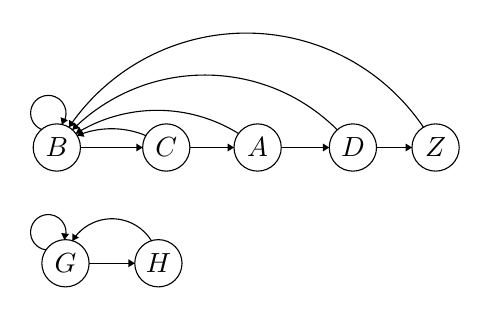
\begin{tikzpicture}[scale=0.1]
\tikzstyle{every node}+=[inner sep=0pt]
\draw [black] (16.6,-25) circle (3);
\draw (16.6,-25) node {$B$};
\draw [black] (30.5,-25) circle (3);
\draw (30.5,-25) node {$C$};
\draw [black] (42.1,-25) circle (3);
\draw (42.1,-25) node {$A$};
\draw [black] (54.2,-25) circle (3);
\draw (54.2,-25) node {$D$};
\draw [black] (64.7,-25) circle (3);
\draw (64.7,-25) node {$Z$};
\draw [black] (17.7,-39.7) circle (3);
\draw (17.7,-39.7) node {$G$};
\draw [black] (29.5,-39.7) circle (3);
\draw (29.5,-39.7) node {$H$};
\draw [black] (19.6,-25) -- (27.5,-25);
\fill [black] (27.5,-25) -- (26.7,-24.5) -- (26.7,-25.5);
\draw [black] (33.5,-25) -- (39.1,-25);
\fill [black] (39.1,-25) -- (38.3,-24.5) -- (38.3,-25.5);
\draw [black] (45.1,-25) -- (51.2,-25);
\fill [black] (51.2,-25) -- (50.4,-24.5) -- (50.4,-25.5);
\draw [black] (57.2,-25) -- (61.7,-25);
\fill [black] (61.7,-25) -- (60.9,-24.5) -- (60.9,-25.5);
\draw [black] (18.139,-22.427) arc (145.95258:34.04742:27.168);
\fill [black] (18.14,-22.43) -- (19,-22.04) -- (18.17,-21.48);
\draw [black] (18.584,-22.753) arc (134.9433:45.0567:23.804);
\fill [black] (18.58,-22.75) -- (19.5,-22.54) -- (18.8,-21.83);
\draw [black] (19.017,-23.227) arc (121.86914:58.13086:19.571);
\fill [black] (19.02,-23.23) -- (19.96,-23.23) -- (19.43,-22.38);
\draw [black] (19.182,-23.491) arc (112.71006:67.28994:11.313);
\fill [black] (19.18,-23.49) -- (20.11,-23.64) -- (19.73,-22.72);
\draw [black] (20.7,-39.7) -- (26.5,-39.7);
\fill [black] (26.5,-39.7) -- (25.7,-39.2) -- (25.7,-40.2);
\draw [black] (14.674,-22.715) arc (247.85512:-40.14488:2.25);
\fill [black] (17.24,-22.08) -- (18.01,-21.53) -- (17.08,-21.15);
\draw [black] (18.568,-36.862) arc (148.44737:31.55263:5.905);
\fill [black] (18.57,-36.86) -- (19.41,-36.44) -- (18.56,-35.92);
\draw [black] (15.244,-37.998) arc (263.00567:-24.99433:2.25);
\fill [black] (17.56,-36.72) -- (18.15,-35.98) -- (17.16,-35.86);
\end{tikzpicture}
\end{center}

\noindent Union by weight:

\begin{center}
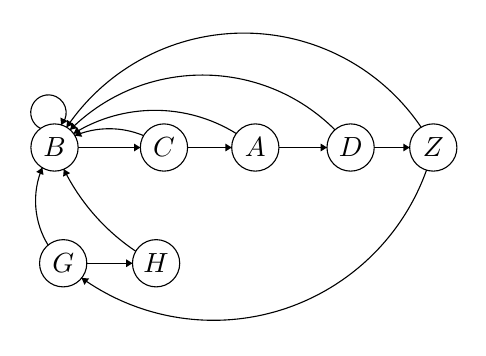
\begin{tikzpicture}[scale=0.1]
\tikzstyle{every node}+=[inner sep=0pt]
\draw [black] (16.6,-25) circle (3);
\draw (16.6,-25) node {$B$};
\draw [black] (30.5,-25) circle (3);
\draw (30.5,-25) node {$C$};
\draw [black] (42.1,-25) circle (3);
\draw (42.1,-25) node {$A$};
\draw [black] (54.2,-25) circle (3);
\draw (54.2,-25) node {$D$};
\draw [black] (64.7,-25) circle (3);
\draw (64.7,-25) node {$Z$};
\draw [black] (17.7,-39.7) circle (3);
\draw (17.7,-39.7) node {$G$};
\draw [black] (29.5,-39.7) circle (3);
\draw (29.5,-39.7) node {$H$};
\draw [black] (18.139,-22.427) arc (145.95258:34.04742:27.168);
\fill [black] (18.14,-22.43) -- (19,-22.04) -- (18.17,-21.48);
\draw [black] (18.584,-22.753) arc (134.9433:45.0567:23.804);
\fill [black] (18.58,-22.75) -- (19.5,-22.54) -- (18.8,-21.83);
\draw [black] (19.017,-23.227) arc (121.86914:58.13086:19.571);
\fill [black] (19.02,-23.23) -- (19.96,-23.23) -- (19.43,-22.38);
\draw [black] (19.182,-23.491) arc (112.71006:67.28994:11.313);
\fill [black] (19.18,-23.49) -- (20.11,-23.64) -- (19.73,-22.72);
\draw [black] (14.838,-22.587) arc (243.86581:-44.13419:2.25);
\fill [black] (17.44,-22.13) -- (18.25,-21.64) -- (17.35,-21.19);
\draw [black] (63.84,-27.873) arc (-19.65614:-125.60805:28.739);
\fill [black] (20.04,-41.57) -- (20.4,-42.44) -- (20.99,-41.63);
\draw [black] (15.789,-37.4) arc (-148.29163:-203.14944:10.713);
\fill [black] (15.05,-27.56) -- (14.28,-28.1) -- (15.2,-28.49);
\draw [black] (26.919,-38.173) arc (-123.80838:-153.65441:26.907);
\fill [black] (17.78,-27.76) -- (17.69,-28.7) -- (18.58,-28.25);
\draw [black] (20.7,-39.7) -- (26.5,-39.7);
\fill [black] (26.5,-39.7) -- (25.7,-39.2) -- (25.7,-40.2);
\draw [black] (19.6,-25) -- (27.5,-25);
\fill [black] (27.5,-25) -- (26.7,-24.5) -- (26.7,-25.5);
\draw [black] (33.5,-25) -- (39.1,-25);
\fill [black] (39.1,-25) -- (38.3,-24.5) -- (38.3,-25.5);
\draw [black] (45.1,-25) -- (51.2,-25);
\fill [black] (51.2,-25) -- (50.4,-24.5) -- (50.4,-25.5);
\draw [black] (57.2,-25) -- (61.7,-25);
\fill [black] (61.7,-25) -- (60.9,-24.5) -- (60.9,-25.5);
\end{tikzpicture}
\end{center}

\noindent Trees:

\begin{center}
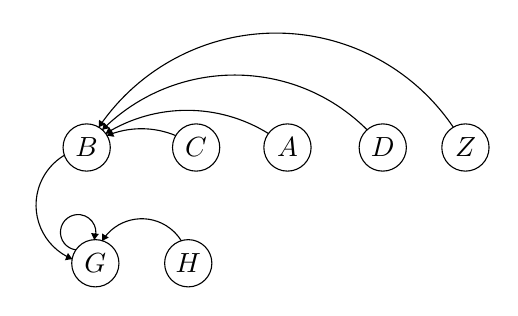
\begin{tikzpicture}[scale=0.1]
\tikzstyle{every node}+=[inner sep=0pt]
\draw [black] (16.6,-25) circle (3);
\draw (16.6,-25) node {$B$};
\draw [black] (30.5,-25) circle (3);
\draw (30.5,-25) node {$C$};
\draw [black] (42.1,-25) circle (3);
\draw (42.1,-25) node {$A$};
\draw [black] (54.2,-25) circle (3);
\draw (54.2,-25) node {$D$};
\draw [black] (64.7,-25) circle (3);
\draw (64.7,-25) node {$Z$};
\draw [black] (17.7,-39.7) circle (3);
\draw (17.7,-39.7) node {$G$};
\draw [black] (29.5,-39.7) circle (3);
\draw (29.5,-39.7) node {$H$};
\draw [black] (18.139,-22.427) arc (145.95258:34.04742:27.168);
\fill [black] (18.14,-22.43) -- (19,-22.04) -- (18.17,-21.48);
\draw [black] (18.584,-22.753) arc (134.9433:45.0567:23.804);
\fill [black] (18.58,-22.75) -- (19.5,-22.54) -- (18.8,-21.83);
\draw [black] (19.017,-23.227) arc (121.86914:58.13086:19.571);
\fill [black] (19.02,-23.23) -- (19.96,-23.23) -- (19.43,-22.38);
\draw [black] (19.182,-23.491) arc (112.71006:67.28994:11.313);
\fill [black] (19.18,-23.49) -- (20.11,-23.64) -- (19.73,-22.72);
\draw [black] (18.568,-36.862) arc (148.44737:31.55263:5.905);
\fill [black] (18.57,-36.86) -- (19.41,-36.44) -- (18.56,-35.92);
\draw [black] (15.244,-37.998) arc (263.00567:-24.99433:2.25);
\fill [black] (17.56,-36.72) -- (18.15,-35.98) -- (17.16,-35.86);
\draw [black] (14.77,-39.157) arc (-112.13943:-239.30164:7.382);
\fill [black] (14.77,-39.16) -- (14.22,-38.39) -- (13.84,-39.32);
\end{tikzpicture}
\end{center}

\noindent Union by weight with trees (larger tree becomes root - $B \;vs.\; G$):

\begin{center}
\begin{tabular}{l @{ vs. } l}

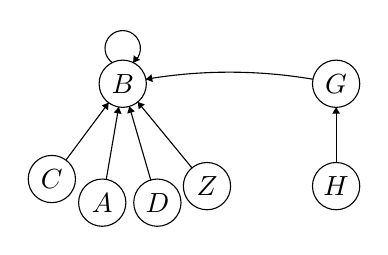
\begin{tikzpicture}[scale=0.1,baseline={(current bounding box.center)}]
\tikzstyle{every node}+=[inner sep=0pt]
\draw [black] (19.9,-20.4) circle (3);
\draw (19.9,-20.4) node {$B$};
\draw [black] (10.9,-32.5) circle (3);
\draw (10.9,-32.5) node {$C$};
\draw [black] (17.3,-35.5) circle (3);
\draw (17.3,-35.5) node {$A$};
\draw [black] (24.3,-35.5) circle (3);
\draw (24.3,-35.5) node {$D$};
\draw [black] (30.6,-33.4) circle (3);
\draw (30.6,-33.4) node {$Z$};
\draw [black] (47,-20.4) circle (3);
\draw (47,-20.4) node {$G$};
\draw [black] (47,-33.4) circle (3);
\draw (47,-33.4) node {$H$};
\draw [black] (12.69,-30.09) -- (18.11,-22.81);
\fill [black] (18.11,-22.81) -- (17.23,-23.15) -- (18.03,-23.75);
\draw [black] (17.81,-32.54) -- (19.39,-23.36);
\fill [black] (19.39,-23.36) -- (18.76,-24.06) -- (19.75,-24.23);
\draw [black] (23.46,-32.62) -- (20.74,-23.28);
\fill [black] (20.74,-23.28) -- (20.48,-24.19) -- (21.44,-23.91);
\draw [black] (28.69,-31.08) -- (21.81,-22.72);
\fill [black] (21.81,-22.72) -- (21.93,-23.65) -- (22.7,-23.02);
\draw [black] (47,-30.4) -- (47,-23.4);
\fill [black] (47,-23.4) -- (46.5,-24.2) -- (47.5,-24.2);
\draw [black] (22.844,-19.826) arc (99.67278:80.32722:63.122);
\fill [black] (22.84,-19.83) -- (23.72,-20.18) -- (23.55,-19.2);
\draw [black] (18.577,-17.72) arc (234:-54:2.25);
\fill [black] (21.22,-17.72) -- (22.1,-17.37) -- (21.29,-16.78);
\end{tikzpicture} &

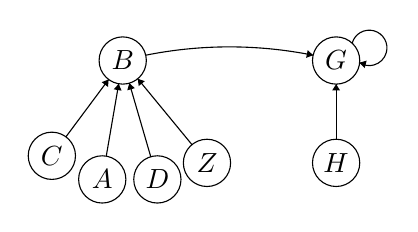
\begin{tikzpicture}[scale=0.1,baseline={(current bounding box.center)}]
\tikzstyle{every node}+=[inner sep=0pt]
\draw [black] (19.9,-20.4) circle (3);
\draw (19.9,-20.4) node {$B$};
\draw [black] (10.9,-32.5) circle (3);
\draw (10.9,-32.5) node {$C$};
\draw [black] (17.3,-35.5) circle (3);
\draw (17.3,-35.5) node {$A$};
\draw [black] (24.3,-35.5) circle (3);
\draw (24.3,-35.5) node {$D$};
\draw [black] (30.6,-33.4) circle (3);
\draw (30.6,-33.4) node {$Z$};
\draw [black] (47,-20.4) circle (3);
\draw (47,-20.4) node {$G$};
\draw [black] (47,-33.4) circle (3);
\draw (47,-33.4) node {$H$};
\draw [black] (12.69,-30.09) -- (18.11,-22.81);
\fill [black] (18.11,-22.81) -- (17.23,-23.15) -- (18.03,-23.75);
\draw [black] (17.81,-32.54) -- (19.39,-23.36);
\fill [black] (19.39,-23.36) -- (18.76,-24.06) -- (19.75,-24.23);
\draw [black] (23.46,-32.62) -- (20.74,-23.28);
\fill [black] (20.74,-23.28) -- (20.48,-24.19) -- (21.44,-23.91);
\draw [black] (28.69,-31.08) -- (21.81,-22.72);
\fill [black] (21.81,-22.72) -- (21.93,-23.65) -- (22.7,-23.02);
\draw [black] (47,-30.4) -- (47,-23.4);
\fill [black] (47,-23.4) -- (46.5,-24.2) -- (47.5,-24.2);
\draw [black] (49.033,-18.21) arc (164.85446:-123.14554:2.25);
\fill [black] (49.97,-20.68) -- (50.62,-21.37) -- (50.88,-20.41);
\draw [black] (22.823,-19.727) arc (101.37486:78.62514:53.882);
\fill [black] (44.08,-19.73) -- (43.39,-19.08) -- (43.19,-20.06);
\end{tikzpicture} \\

\end{tabular}
\end{center}

\begin{lstlisting}[mathescape]
if Find-Set($u_i$) != Find-Set($v_i$):
	union($u_i,v_i$)
	$T \leftarrow U \cup \{(u_i,v_i)\}$
\end{lstlisting}

\newpage
\noindent Path compression:

\begin{center}
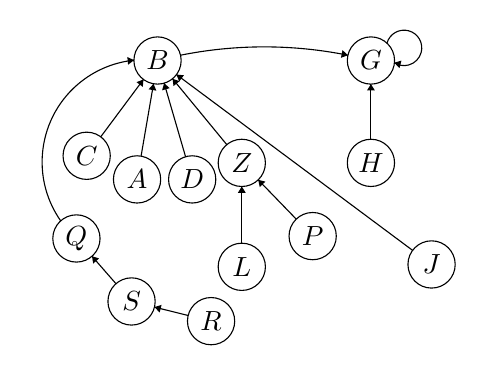
\begin{tikzpicture}[scale=0.1]
\tikzstyle{every node}+=[inner sep=0pt]
\draw [black] (19.9,-20.4) circle (3);
\draw (19.9,-20.4) node {$B$};
\draw [black] (10.9,-32.5) circle (3);
\draw (10.9,-32.5) node {$C$};
\draw [black] (17.3,-35.5) circle (3);
\draw (17.3,-35.5) node {$A$};
\draw [black] (24.3,-35.5) circle (3);
\draw (24.3,-35.5) node {$D$};
\draw [black] (30.6,-33.4) circle (3);
\draw (30.6,-33.4) node {$Z$};
\draw [black] (47,-20.4) circle (3);
\draw (47,-20.4) node {$G$};
\draw [black] (47,-33.4) circle (3);
\draw (47,-33.4) node {$H$};
\draw [black] (30.6,-46.6) circle (3);
\draw (30.6,-46.6) node {$L$};
\draw [black] (39.6,-42.7) circle (3);
\draw (39.6,-42.7) node {$P$};
\draw [black] (54.7,-46.3) circle (3);
\draw (54.7,-46.3) node {$J$};
\draw [black] (9.6,-43) circle (3);
\draw (9.6,-43) node {$Q$};
\draw [black] (16.6,-51) circle (3);
\draw (16.6,-51) node {$S$};
\draw [black] (26.7,-53.5) circle (3);
\draw (26.7,-53.5) node {$R$};
\draw [black] (12.69,-30.09) -- (18.11,-22.81);
\fill [black] (18.11,-22.81) -- (17.23,-23.15) -- (18.03,-23.75);
\draw [black] (17.81,-32.54) -- (19.39,-23.36);
\fill [black] (19.39,-23.36) -- (18.76,-24.06) -- (19.75,-24.23);
\draw [black] (23.46,-32.62) -- (20.74,-23.28);
\fill [black] (20.74,-23.28) -- (20.48,-24.19) -- (21.44,-23.91);
\draw [black] (28.69,-31.08) -- (21.81,-22.72);
\fill [black] (21.81,-22.72) -- (21.93,-23.65) -- (22.7,-23.02);
\draw [black] (47,-30.4) -- (47,-23.4);
\fill [black] (47,-23.4) -- (46.5,-24.2) -- (47.5,-24.2);
\draw [black] (49.033,-18.21) arc (164.85446:-123.14554:2.25);
\fill [black] (49.97,-20.68) -- (50.62,-21.37) -- (50.88,-20.41);
\draw [black] (22.823,-19.727) arc (101.37486:78.62514:53.882);
\fill [black] (44.08,-19.73) -- (43.39,-19.08) -- (43.19,-20.06);
\draw [black] (30.6,-43.6) -- (30.6,-36.4);
\fill [black] (30.6,-36.4) -- (30.1,-37.2) -- (31.1,-37.2);
\draw [black] (37.51,-40.54) -- (32.69,-35.56);
\fill [black] (32.69,-35.56) -- (32.88,-36.48) -- (33.6,-35.78);
\draw [black] (52.29,-44.51) -- (22.31,-22.19);
\fill [black] (22.31,-22.19) -- (22.65,-23.07) -- (23.25,-22.27);
\draw [black] (7.608,-40.766) arc (-144.8853:-264.11716:12.997);
\fill [black] (16.91,-20.36) -- (16.06,-19.95) -- (16.16,-20.94);
\draw [black] (14.62,-48.74) -- (11.58,-45.26);
\fill [black] (11.58,-45.26) -- (11.73,-46.19) -- (12.48,-45.53);
\draw [black] (23.79,-52.78) -- (19.51,-51.72);
\fill [black] (19.51,-51.72) -- (20.17,-52.4) -- (20.41,-51.43);
\end{tikzpicture}
\end{center}

\noindent \texttt{Find-Set($P$)}:

\begin{center}
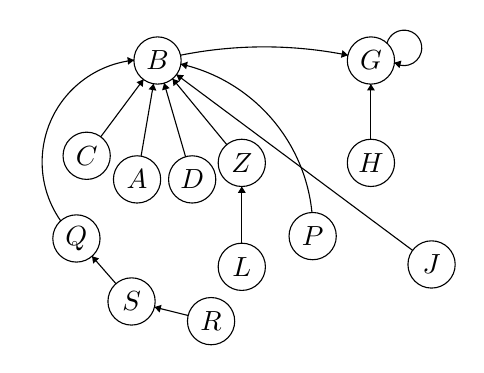
\begin{tikzpicture}[scale=0.1]
\tikzstyle{every node}+=[inner sep=0pt]
\draw [black] (19.9,-20.4) circle (3);
\draw (19.9,-20.4) node {$B$};
\draw [black] (10.9,-32.5) circle (3);
\draw (10.9,-32.5) node {$C$};
\draw [black] (17.3,-35.5) circle (3);
\draw (17.3,-35.5) node {$A$};
\draw [black] (24.3,-35.5) circle (3);
\draw (24.3,-35.5) node {$D$};
\draw [black] (30.6,-33.4) circle (3);
\draw (30.6,-33.4) node {$Z$};
\draw [black] (47,-20.4) circle (3);
\draw (47,-20.4) node {$G$};
\draw [black] (47,-33.4) circle (3);
\draw (47,-33.4) node {$H$};
\draw [black] (30.6,-46.6) circle (3);
\draw (30.6,-46.6) node {$L$};
\draw [black] (39.6,-42.7) circle (3);
\draw (39.6,-42.7) node {$P$};
\draw [black] (54.7,-46.3) circle (3);
\draw (54.7,-46.3) node {$J$};
\draw [black] (9.6,-43) circle (3);
\draw (9.6,-43) node {$Q$};
\draw [black] (16.6,-51) circle (3);
\draw (16.6,-51) node {$S$};
\draw [black] (26.7,-53.5) circle (3);
\draw (26.7,-53.5) node {$R$};
\draw [black] (12.69,-30.09) -- (18.11,-22.81);
\fill [black] (18.11,-22.81) -- (17.23,-23.15) -- (18.03,-23.75);
\draw [black] (17.81,-32.54) -- (19.39,-23.36);
\fill [black] (19.39,-23.36) -- (18.76,-24.06) -- (19.75,-24.23);
\draw [black] (23.46,-32.62) -- (20.74,-23.28);
\fill [black] (20.74,-23.28) -- (20.48,-24.19) -- (21.44,-23.91);
\draw [black] (28.69,-31.08) -- (21.81,-22.72);
\fill [black] (21.81,-22.72) -- (21.93,-23.65) -- (22.7,-23.02);
\draw [black] (47,-30.4) -- (47,-23.4);
\fill [black] (47,-23.4) -- (46.5,-24.2) -- (47.5,-24.2);
\draw [black] (49.033,-18.21) arc (164.85446:-123.14554:2.25);
\fill [black] (49.97,-20.68) -- (50.62,-21.37) -- (50.88,-20.41);
\draw [black] (22.823,-19.727) arc (101.37486:78.62514:53.882);
\fill [black] (44.08,-19.73) -- (43.39,-19.08) -- (43.19,-20.06);
\draw [black] (30.6,-43.6) -- (30.6,-36.4);
\fill [black] (30.6,-36.4) -- (30.1,-37.2) -- (31.1,-37.2);
\draw [black] (52.29,-44.51) -- (22.31,-22.19);
\fill [black] (22.31,-22.19) -- (22.65,-23.07) -- (23.25,-22.27);
\draw [black] (7.608,-40.766) arc (-144.8853:-264.11716:12.997);
\fill [black] (16.91,-20.36) -- (16.06,-19.95) -- (16.16,-20.94);
\draw [black] (14.62,-48.74) -- (11.58,-45.26);
\fill [black] (11.58,-45.26) -- (11.73,-46.19) -- (12.48,-45.53);
\draw [black] (23.79,-52.78) -- (19.51,-51.72);
\fill [black] (19.51,-51.72) -- (20.17,-52.4) -- (20.41,-51.43);
\draw [black] (22.862,-20.857) arc (77.22701:5.68827:21.511);
\fill [black] (22.86,-20.86) -- (23.53,-21.52) -- (23.75,-20.55);
\end{tikzpicture}
\end{center}

\noindent \texttt{Find-Set($S$)}:

\begin{center}
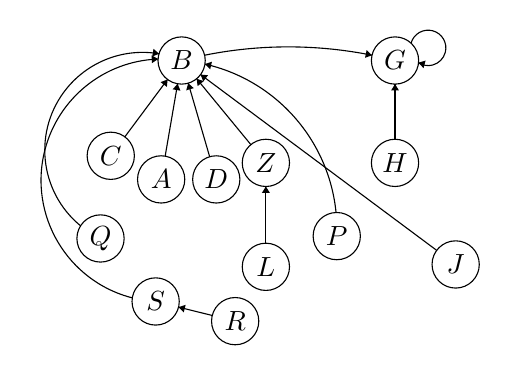
\begin{tikzpicture}[scale=0.1]
\tikzstyle{every node}+=[inner sep=0pt]
\draw [black] (19.9,-20.4) circle (3);
\draw (19.9,-20.4) node {$B$};
\draw [black] (10.9,-32.5) circle (3);
\draw (10.9,-32.5) node {$C$};
\draw [black] (17.3,-35.5) circle (3);
\draw (17.3,-35.5) node {$A$};
\draw [black] (24.3,-35.5) circle (3);
\draw (24.3,-35.5) node {$D$};
\draw [black] (30.6,-33.4) circle (3);
\draw (30.6,-33.4) node {$Z$};
\draw [black] (47,-20.4) circle (3);
\draw (47,-20.4) node {$G$};
\draw [black] (47,-33.4) circle (3);
\draw (47,-33.4) node {$H$};
\draw [black] (30.6,-46.6) circle (3);
\draw (30.6,-46.6) node {$L$};
\draw [black] (39.6,-42.7) circle (3);
\draw (39.6,-42.7) node {$P$};
\draw [black] (54.7,-46.3) circle (3);
\draw (54.7,-46.3) node {$J$};
\draw [black] (9.6,-43) circle (3);
\draw (9.6,-43) node {$Q$};
\draw [black] (16.6,-51) circle (3);
\draw (16.6,-51) node {$S$};
\draw [black] (26.7,-53.5) circle (3);
\draw (26.7,-53.5) node {$R$};
\draw [black] (12.69,-30.09) -- (18.11,-22.81);
\fill [black] (18.11,-22.81) -- (17.23,-23.15) -- (18.03,-23.75);
\draw [black] (17.81,-32.54) -- (19.39,-23.36);
\fill [black] (19.39,-23.36) -- (18.76,-24.06) -- (19.75,-24.23);
\draw [black] (23.46,-32.62) -- (20.74,-23.28);
\fill [black] (20.74,-23.28) -- (20.48,-24.19) -- (21.44,-23.91);
\draw [black] (28.69,-31.08) -- (21.81,-22.72);
\fill [black] (21.81,-22.72) -- (21.93,-23.65) -- (22.7,-23.02);
\draw [black] (47,-30.4) -- (47,-23.4);
\fill [black] (47,-23.4) -- (46.5,-24.2) -- (47.5,-24.2);
\draw [black] (49.033,-18.21) arc (164.85446:-123.14554:2.25);
\fill [black] (49.97,-20.68) -- (50.62,-21.37) -- (50.88,-20.41);
\draw [black] (22.823,-19.727) arc (101.37486:78.62514:53.882);
\fill [black] (44.08,-19.73) -- (43.39,-19.08) -- (43.19,-20.06);
\draw [black] (30.6,-43.6) -- (30.6,-36.4);
\fill [black] (30.6,-36.4) -- (30.1,-37.2) -- (31.1,-37.2);
\draw [black] (52.29,-44.51) -- (22.31,-22.19);
\fill [black] (22.31,-22.19) -- (22.65,-23.07) -- (23.25,-22.27);
\draw [black] (7.073,-41.397) arc (-129.30413:-279.69833:12.42);
\fill [black] (17.03,-19.54) -- (16.33,-18.92) -- (16.16,-19.9);
\draw [black] (23.79,-52.78) -- (19.51,-51.72);
\fill [black] (19.51,-51.72) -- (20.17,-52.4) -- (20.41,-51.43);
\draw [black] (22.862,-20.857) arc (77.22701:5.68827:21.511);
\fill [black] (22.86,-20.86) -- (23.53,-21.52) -- (23.75,-20.55);
\draw [black] (13.64,-50.544) arc (-104.33804:-267.9723:15.409);
\fill [black] (16.91,-20.21) -- (16.09,-19.74) -- (16.13,-20.74);
\end{tikzpicture}
\end{center}

\subsection*{Union by Rank}

\begin{itemize}
	\item upper bound on height
\end{itemize}

\begin{center}
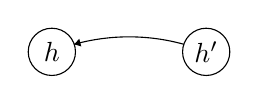
\begin{tikzpicture}[scale=0.1]
\tikzstyle{every node}+=[inner sep=0pt]
\draw [black] (23.8,-26.3) circle (3);
\draw (23.8,-26.3) node {$h$};
\draw [black] (43.4,-26.3) circle (3);
\draw (43.4,-26.3) node {$h'$};
\draw [black] (26.64,-25.337) arc (105.4454:74.5546:26.136);
\fill [black] (26.64,-25.34) -- (27.54,-25.61) -- (27.28,-24.64);
\end{tikzpicture}
\end{center}

\begin{equation*}
\begin{split}
	h' < h & \rightarrow h \\
	h' = h & \rightarrow h + 1 \\
\end{split}
\end{equation*}

\subsection*{Trees with Union by Rank + Path Compression}

\noindent \texttt{Make-Set($x$)}: rank$_x$ = 0,

\begin{center}
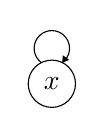
\begin{tikzpicture}[scale=0.1]
\tikzstyle{every node}+=[inner sep=0pt]
\draw [black] (43.4,-26.3) circle (3);
\draw (43.4,-26.3) node {$x$};
\draw [black] (42.077,-23.62) arc (234:-54:2.25);
\fill [black] (44.72,-23.62) -- (45.6,-23.27) -- (44.79,-22.68);
\end{tikzpicture}
\end{center}

\noindent \texttt{Union($x,y$)}: the root with higher rank becomes the new root and is unchanged. If two ranks are equal, either root is chosen as new root and rank is incremented. \\

\noindent \texttt{Find-Set($x$)}: use path compression and leave ranks unchanged \\

\noindent It is possible to prove that the worst-case running time for a sequence of $m$ operations where there are are $n$ \texttt{Make-Set} operations is $O(m \log*(n))$ or $O(m \alpha(n))$.

$$ log* n = \left \{ \begin{array}{l l}
	0 & \quad 0 \leq n \leq 2 \\
	1 & \quad n=3 \\
	2 & \quad 4 \leq n \leq 7 \\
	3 & \quad 8 \leq n \leq 2047 \\
	4 & \quad 2048 \leq n \leq i \textrm{ where } i > 10^{80} \\
\end{array} \right . $$

\end{document}
